\documentclass[11pt,english,compress]{beamer}
\usepackage[utf8]{inputenc}
\usepackage{verbatim}
\usepackage{eurosym}
\usepackage{ stmaryrd }
\usepackage{subfig}

\useoutertheme{smoothbars}
\useinnertheme[shadow=true]{rounded}
\usecolortheme{orchid}
\usecolortheme{whale}
\title{EzBench, a tool to help you benchmark and bisect the Graphics Stack's performance}
\subtitle{}
\author{Martin Peres}
\institute{Intel Open Source Technology Center Finland}

\AtBeginSection[]{
  \begin{frame}{Summary}
  \small \tableofcontents[currentsection, hideothersubsections]
  \end{frame} 
}

\begin{document}

\setbeamertemplate{navigation symbols}{}

\begin{frame}
	\titlepage
\end{frame}

\section{Introduction}
\subsection*{Introduction}
\begin{frame}
	\frametitle{Introduction}

	\begin{block}{Current situation}
		\begin{itemize}
			\item Complex games/benchmarks are available and used on Linux;
			\item Drivers are getting more complex as performance improves;
			\item Users now rely on Open Source drivers for games/other...
		\end{itemize}
	\end{block}
	
	\pause
	
	\begin{block}{Risks when merging new code}
		\begin{itemize}
			\item Break previous functionalities / rendering;
			\item Break the performance of a game inadvertly;
			\item Improve the performance of one game but slow down others.
		\end{itemize}
	\end{block}
	
	\pause
	
	\begin{block}{}
		$\Rightarrow$ Need to test and benchmark all the platforms and games of interest.
	\end{block}
\end{frame}

\section{Graphics Continuous Integration}
\subsection*{Objectives}
\begin{frame}
	\frametitle{CI: Objectives and chalenges}
	
	\begin{block}{Objectives}
		\begin{itemize}
			\item Catch changes in unit tests, rendering, performance or power;
			\item Pin-point the change, to help bug-reporting and fixing;
			\item Guarantee reproducibility of the results;
			\item Warn the relevant developers of changes.
		\end{itemize}
	\end{block}
	
	\pause
	
	\begin{block}{Challenges}
		\begin{itemize}
			\item Unit tests, performance, metrics or rendering can be unstable;
			\item Multiple components interacting with each-other;
			\item Avoid false positives and false negatives;
			\item Impossible to test every commit.
		\end{itemize}
	\end{block}
\end{frame}

\subsection*{Current solutions}
\begin{frame}
	\frametitle{CI: Current tools}
	
	\begin{block}{Current solutions}
		\begin{itemize}
			\item Unit testing: Piglit, dEQP, gl-CTS, vk-CTS, more...;
			\item Performance: Phoronix Test Suite, Sixonix;
			\item Rendering: Phoronix Test Suite, Anholt's trace-db;
			\item Job scheduling: Phoronix Test Suite, Jenkins.
		\end{itemize}
	\end{block}
\end{frame}


\begin{frame}
	\frametitle{Example of variances}
	
	\begin{block}{}
		The variance forces us to execute multiple runs, which takes time!
	\end{block}
	
	\pause
	
	\begin{figure}%
		\centering
		\subfloat[Bad FPS distribution]{{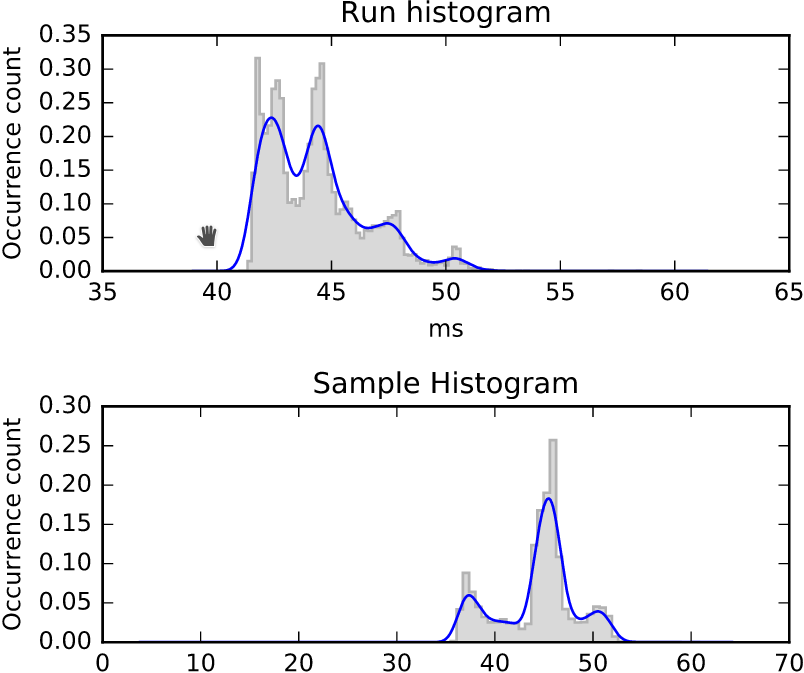
\includegraphics[width=5cm]{variance_bad.png} }}%
		\qquad
		\pause
		\subfloat[Good FPS distribution]{{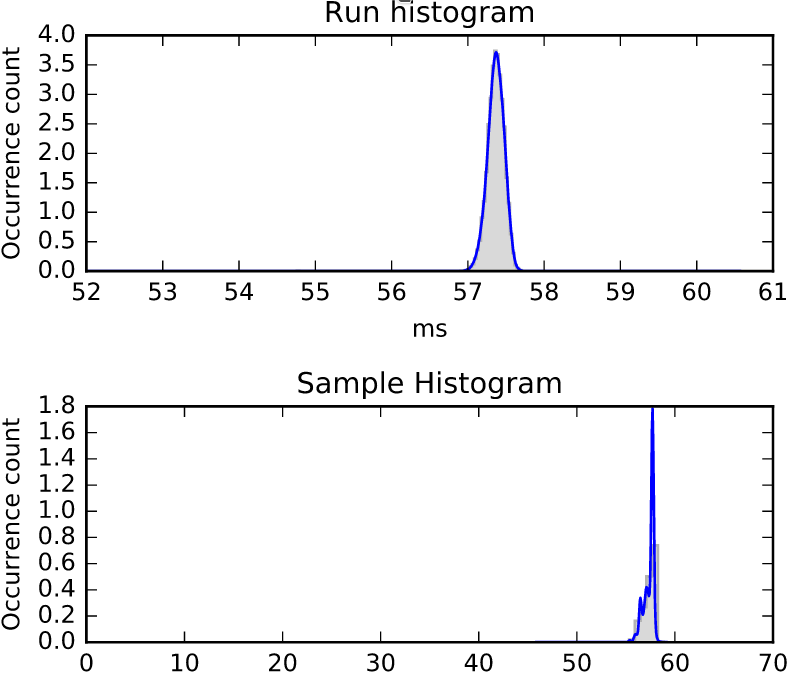
\includegraphics[width=5cm]{variance_good.png} }}%
		\caption{Examples of variance}%
	\end{figure}
\end{frame}

% Summary: Main benefits compared to other tools

\end{document}
